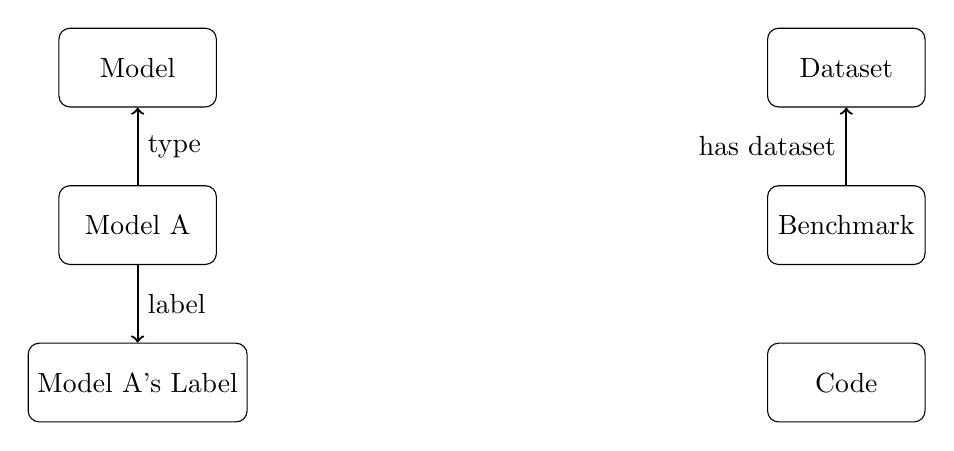
\begin{tikzpicture}[
	node/.style={draw, rounded corners, align=center, minimum width=2cm, minimum height=1cm},
	edge/.style={->, thick},
	scale=1, transform shape
]

% Left side nodes
\node[node] (modelA) at (-4.5, 0) {Model A};
\node[node] (model) at (-4.5, 2) {Model};
\node[node] (label) at (-4.5, -2) {Model A's Label};

% Right side nodes
\node[node] (benchmark) at (4.5, 0) {Benchmark};
\node[node] (dataset) at (4.5, 2) {Dataset};
\node[node] (code) at (4.5, -2) {Code};

% Edges
\draw[edge] (benchmark) -- node[midway, left] {has dataset} (dataset);
\draw[edge] (modelA) -- node[midway, right] {type} (model);
\draw[edge] (modelA) -- node[midway, right] {label} (label);

\end{tikzpicture}
